\documentclass[11pt]{article}
\usepackage[margin=1in]{geometry}
\usepackage{amsmath,amssymb,booktabs,graphicx,microtype,float}
\usepackage[hidelinks]{hyperref}
\newcommand{\E}{\mathbb{E}}

\title{Medium-Entropy SCGF and Rare-Event Sampling Pilot}
\author{}
\date{August 27, 2026}

\begin{document}
\maketitle

\section*{Question and status}

For the boundary-driven NLS chain we estimate the finite-time scaled
cumulant-generating function (SCGF)
\[
  \psi_t(k)=\frac{1}{t}\log\E\!\left[e^{-k\Sigma_t^{\rm m}}\right],
\]
where \(\Sigma_t^{\rm m}\) is the entropy delivered to the reservoirs.  The
long-time Gallavotti--Cohen diagnostic would be
\(\psi(k)=\psi(1-k)\).  The current result is a validated low-tilt pilot, not
a verification of this symmetry: no nontrivial pair \(k\) and \(1-k\) has
simultaneously passed the rare-event support gates.

\section*{Direct million-sample diagnostic}

The direct estimator uses the audited \(1{,}000{,}064\) non-overlapping
\(t=20\) blocks for each \(n=10,20,30,40\), together with their aggregations
through \(t=200\).  A point is accepted only if sample-weight ESS is at least
1000, independent-stream ESS is at least 32 of 128, the largest sample weight
is at most 1\%, and the largest stream weight is at most 10\%.  The independent
audit performed 14,762 checks with no errors.

Near \(k=1\), the direct estimate is controlled by only about 1--8 effective
samples, and a single observation can carry 28\%--96\% of the total
exponential weight.  Therefore the apparent values near \(k=1\) are rejected.
The directly sampled data contain no nontrivial \(k\leftrightarrow1-k\) pair
for which both points pass.

\begin{figure}[ht]
  \centering
  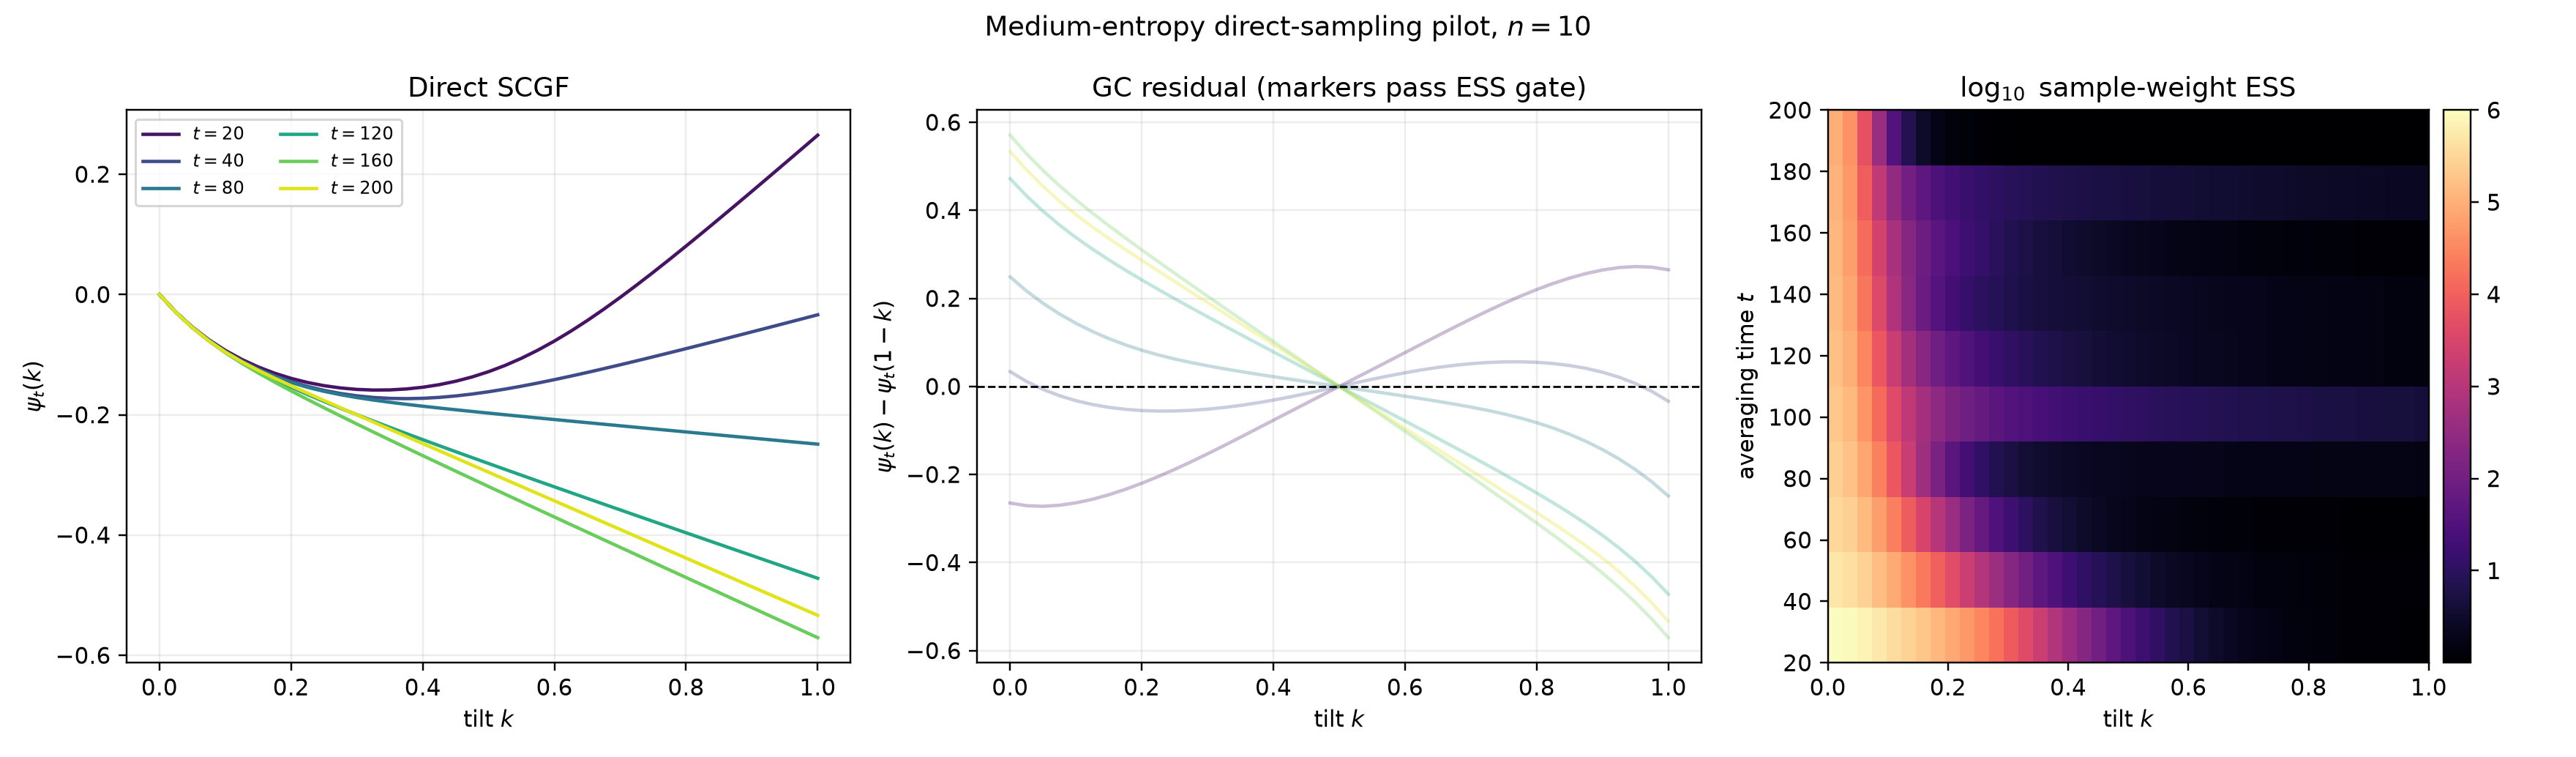
\includegraphics[width=0.92\textwidth]{../direct_pilot/scgf_ess_n10.png}
  \caption{Direct finite-time SCGF and support diagnostics for \(n=10\).
  Exponential reweighting loses effective support well before \(k=1\).}
\end{figure}

\section*{Population-dynamics estimator}

Two equivalent Feynman--Kac implementations were checked.  The naive version
weights each segment by \(e^{-k\Delta\Sigma^{\rm m}}\).  The guided version
uses the corresponding tilted bath drift and scalar potential.  For one bath,
writing \(M=\sum_j|c_j|^2\) and \(F=\nabla E\),
\[
 d\Sigma^{\rm m}
 =\left(\frac{\gamma|F|^2}{T}-4\gamma M\right)dt
 -\sqrt{\frac{2\gamma}{T}}F\cdot dW .
\]
Tilting by \(e^{-k\Sigma^{\rm m}}\) changes the bath drift from
\(-\gamma F\) to \(\gamma(2k-1)F\) and introduces
\[
 V_k=\gamma(k^2-k)\frac{|F|^2}{T}+4\gamma kM
\]
per bath.  Fixed-population systematic resampling is accompanied by
weight-ESS and full ancestry diagnostics.

The exact Gaussian cloning self-test passes.  Four independent \(k=0\) runs
recover the direct stationary medium-entropy rate and action current within
0.54 standard errors.  Over one selection interval, naive and guided
estimators differ by only 0.00290 at \(k=0.1\) and 0.01393 at \(k=0.5\).

\begin{table}[ht]
\centering
\caption{Population convergence at \(n=10\), \(t=20\), \(k=0.3\).}
\begin{tabular}{rrrrr}
\toprule
\(N_c\) & mean \(\psi_{20}(0.3)\) & run SE & min. roots & min. root ESS\\
\midrule
256  & -0.15685 & 0.00884 & 9  & 3.70\\
512  & -0.16985 & 0.01100 & 18 & 9.09\\
1024 & -0.16035 & 0.00513 & 40 & 20.87\\
\bottomrule
\end{tabular}
\end{table}

The direct million-sample value is \(-0.15784\).  The \(N_c=1024\) result is
0.49 independent-run standard errors away.  It passes the predeclared support
gate, and the \(N_c=512\to1024\) change, 0.00950, is smaller than both two
combined standard errors (0.02429) and the absolute tolerance 0.02.
Changing the selection interval from \(\Delta=0.5\) to 0.25 or 1.0 changes
the four-run mean by 0.00869 and 0.00452, respectively.  Both comparisons pass
the predeclared two-standard-error and absolute 0.01 criteria, and every
setting retains at least 35 initial roots.
Halving the timestep gives \(-0.15866\pm0.00324\), compared with
\(-0.16035\pm0.00513\) at \(\Delta t=5\times10^{-4}\).  Their difference,
0.00169, is below two combined standard errors (0.01214) and the absolute 0.01
tolerance.  The fine-step runs have zero midpoint failures and retain at least
39 initial roots.

\begin{figure}[ht]
  \centering
  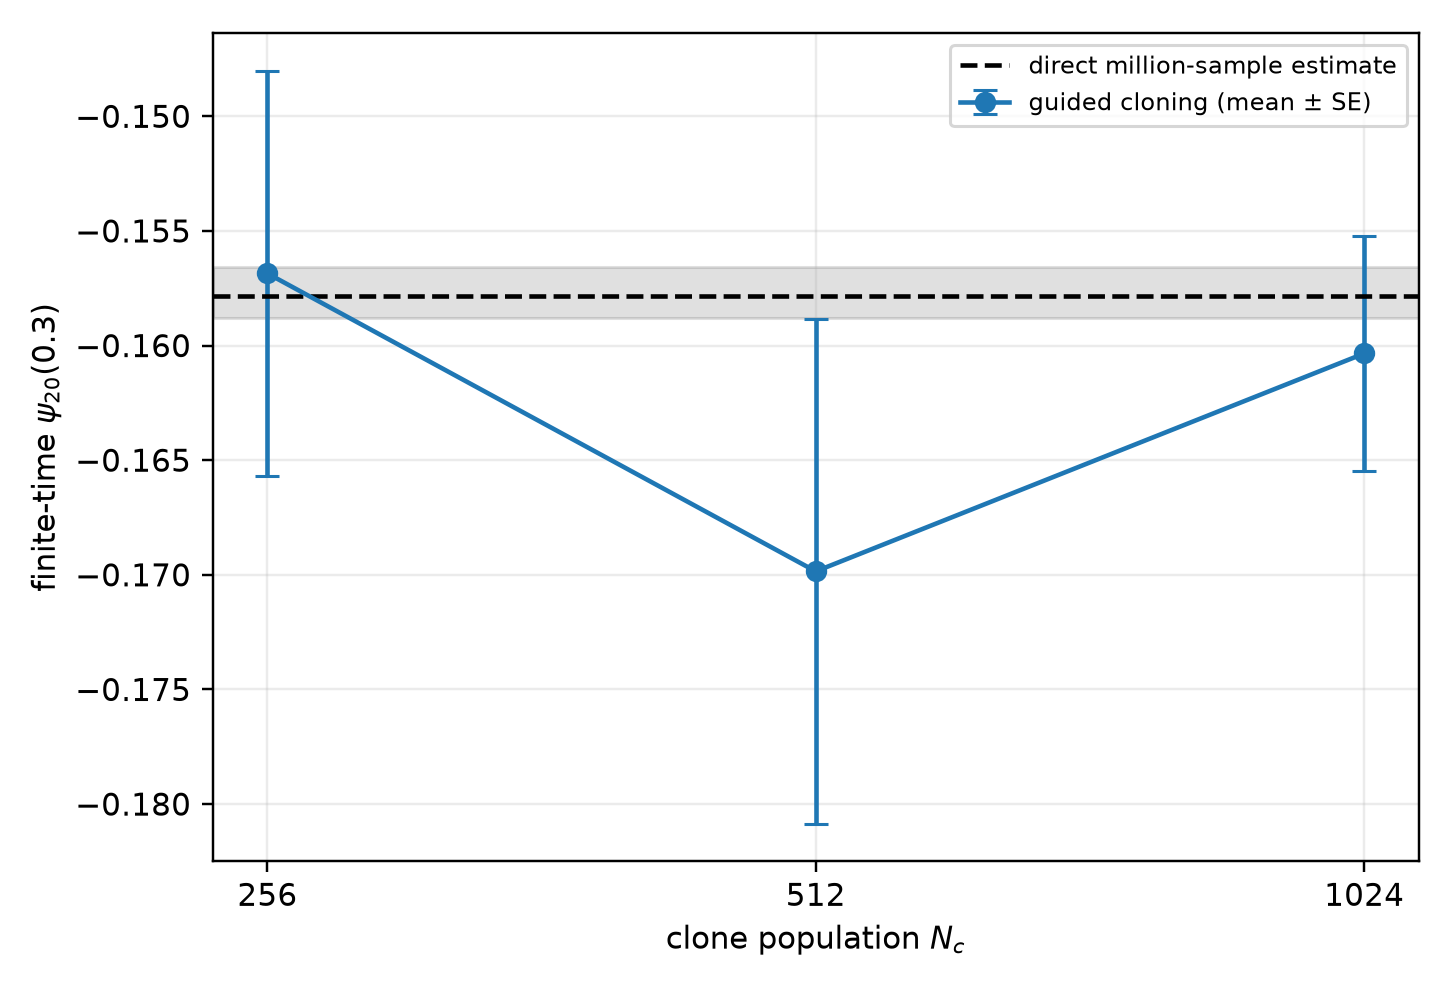
\includegraphics[width=0.76\textwidth]{../aggregate/population_convergence_k0p3.png}
  \caption{Clone-population convergence.  The band is the direct estimator's
  stream-bootstrap confidence interval.}
\end{figure}

\section*{Why the fluctuation-theorem gate remains closed}

For \(k\ge0.5\), the tested populations lose genealogical diversity.  Near
\(k=0.7\), the standard \(N_c=1024\), \(t=20\) attempt produces three
completed replicas, all ending with a single surviving initial root; a fourth
replica is rejected by the midpoint numerical gate before entering the
aggregate.  Extending the accepted \(k=0.3\) setting to \(t=40\) gives
\(\psi_{40}(0.3)=-0.17607\pm0.00719\), but only 14--19 distinct roots remain
and the minimum root ESS is 8.90, below the predeclared requirements of 32 and
16.  These values are excluded.  Consequently no nontrivial
\(k\leftrightarrow1-k\) comparison is available.

This limitation is not evidence against the theorem.  The sampled observable
is medium entropy, whereas the exact finite-time relation concerns total
entropy,
\[
 \Delta s_{\rm tot}=\Sigma_t^{\rm m}
 -\log\rho_{\rm ss}(X_t)+\log\rho_{\rm ss}(X_0).
\]
The stationary-density endpoint is not known for the long chains.  In an
unbounded state space, endpoint-energy fluctuations may also affect
exponential moments near \(k=1\), so ordinary sampling and naive population
growth need not resolve the problem.

\section*{Small-chain total-entropy endpoint control}

As a separate control, we estimate the NESS endpoint density at \(n=2\) in
the reduced coordinates \((\log|c_1|^2,\log|c_2|^2,
2(\arg c_2-\arg c_1))\).  Equal-temperature and driven calculations each use
32,768 non-overlapping \(t=20\) blocks from 64 streams.  All raw formulas and
row counts reproduce independently, no midpoint solve fails, and the
first-law RMS rates are \(1.24\times10^{-5}\) and
\(1.51\times10^{-5}\), respectively.

The smoothing scale is selected using only the first half of the
equal-temperature streams.  On the held-out half, the learned density log
ratio has support 0.9868, slope 0.9296, correlation 0.9675, and RMSE 0.3603
against the exact Gibbs ratio \(\Delta E/T\); these predeclared ordinary-error
gates pass.  The exact Gibbs endpoint also gives
\(\log\langle e^{-\Delta s_{\rm tot}}\rangle=-3.29\times10^{-7}\).

\begin{figure}[H]
  \centering
  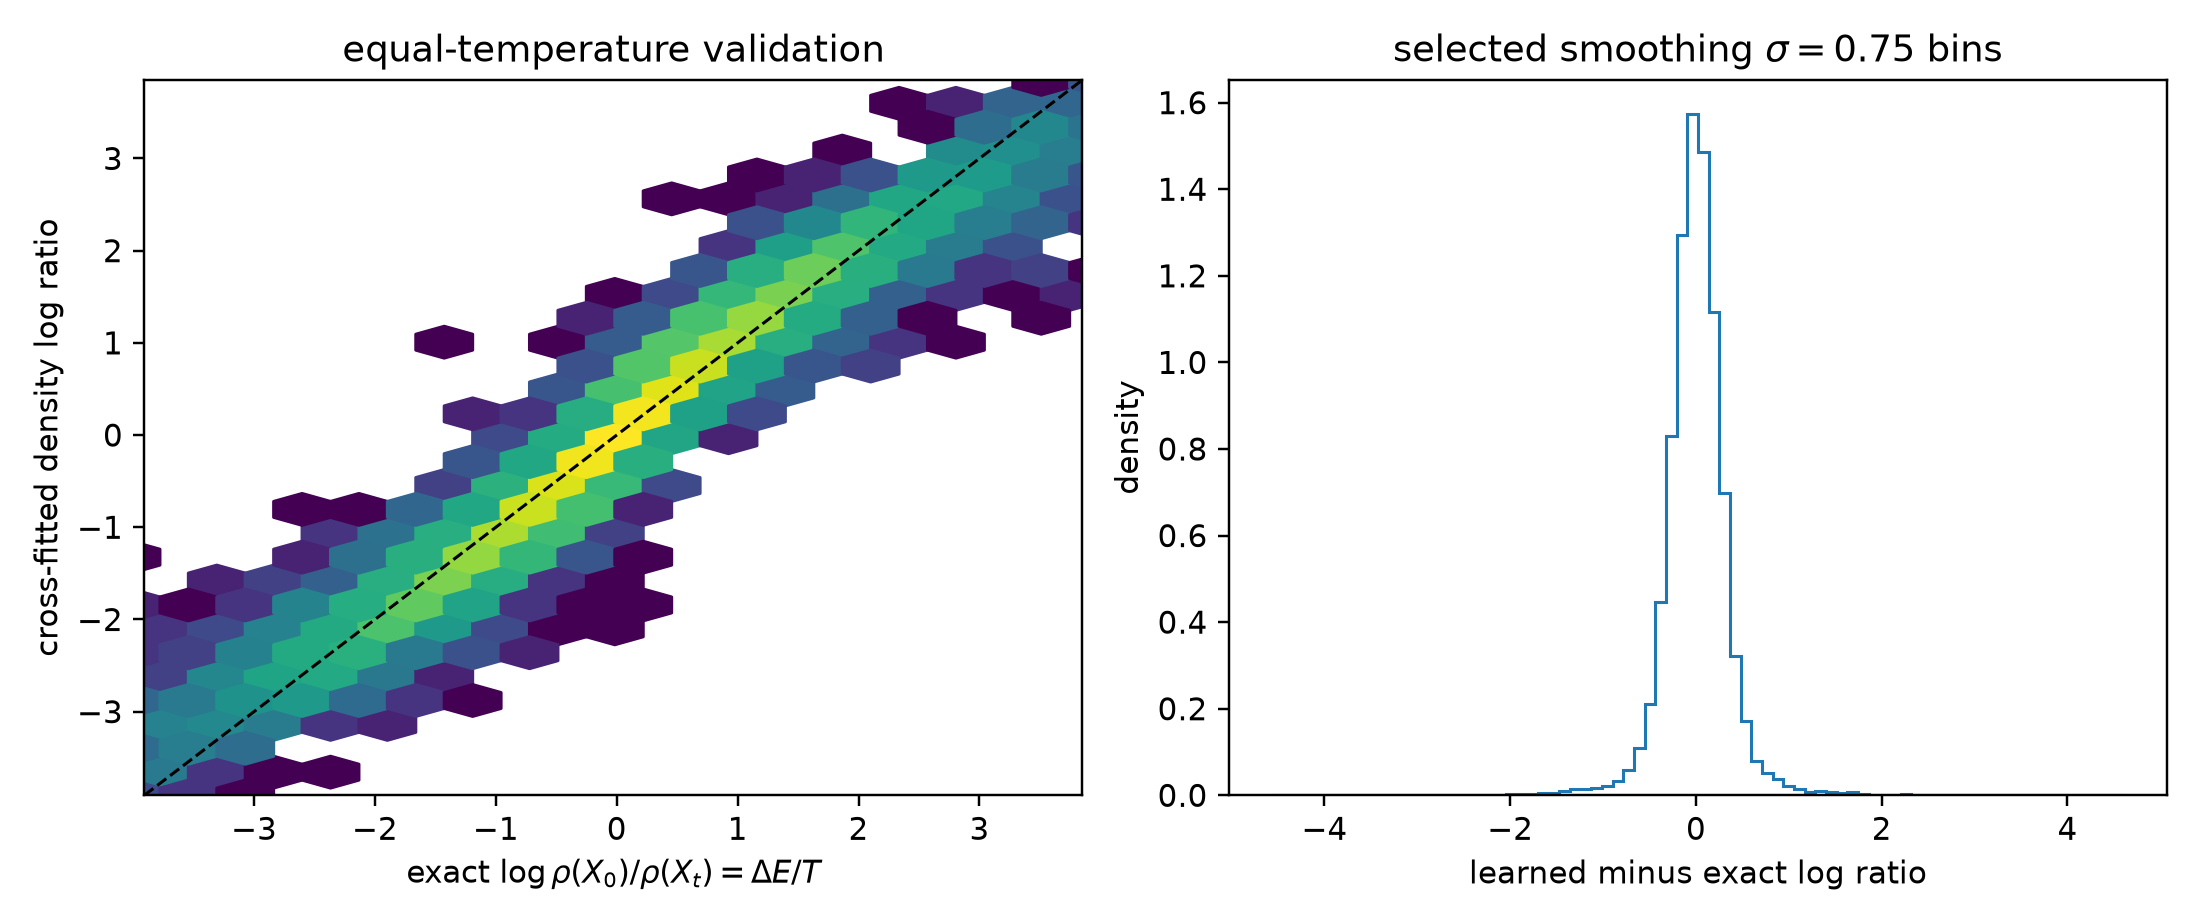
\includegraphics[width=0.88\textwidth]{../total_entropy_n2/analysis/equilibrium_density_validation.png}
  \caption{Held-out equal-temperature validation of the nonparametric
  stationary-density ratio.  Pointwise agreement alone is insufficient for
  an exponential-moment fluctuation test.}
\end{figure}

The more sensitive learned-density integral-FT gate does not pass:
\(\log\langle e^{-\Delta s_{\rm tot}}\rangle=0.0843\), with a stream-bootstrap
95\% interval \([0.0700,0.1025]\).  In the driven data the exponential-weight
ESS is only 1.63, and no positive/negative histogram-bin pair contains at
least 20 raw observations on both sides.  The \(n=2\) total-entropy result is
therefore blocked.  It diagnoses endpoint-density and rare-negative-tail
limitations; it is not evidence against the theorem.

\section*{Conclusion}

Direct and population-dynamics estimators agree in the low-tilt region, and
the \(k=0.3\) point passes independent-run, population, ancestry, and numerical
checks.  The complementary high-tilt region remains rare-event and
boundary-term limited.  The independent \(n=2\) endpoint control also fails
its integral-FT and driven exponential-weight-support gates.  The defensible
conclusion is therefore that the Gallavotti--Cohen symmetry is \emph{not
verified by the present study}; it is neither proved nor shown to be violated.

\end{document}
